\documentclass{article}

%\usepackage{mathtools}
\usepackage{amsfonts}
\usepackage[spanish,mexico]{babel}
\usepackage[utf8]{inputenc}
\usepackage{graphicx}
\usepackage{booktabs}
\usepackage{url}
\usepackage{listings}%http://www.tex.ac.uk/FAQ-codelist.html
\lstset{language=Python}
\graphicspath{ {img/} }
%\usepackage{enumitem}
%\usepackage{tikz}

\title{Densidades y distancias promedio de grafos ciclos a completos}
\author{José Alberto Benavides Vázquez}
\date{\today}

\begin{document}

  \maketitle

  Un \textbf{grafo ciclo} es un grafo en el que sus $n$ nodos están conectados uno tras otro, sin repeticiones, salvo por el úlitmo nodo que se conecta al primero para formar una figura que se asemeja a un polígono de $n$ lados. Por su parte, un \textbf{grafo completo} es un grafo ciclo en el que sus $n$ nodos están conectados con los restantes $n - 1$ nodos. En cuanto a las aristas, los grafos ciclo tienen la mínima cantidad de aristas necesarias para cumplir su definición y formar un ciclo, esto es $a = n$ aristas; mientras que los grafos completos poseen todas las aristas posibles que pueden establecerse sin repetir pares de nodos entre sí, a saber $a = n \cdot (n-1)/2$ aristas. A partir de estas descripciones, se puede definir un valor $k$ que especifique la cantidad de nodos vecinos con los que se conectará cada nodo de este tipo de grafos por cada uno de sus costado. Este valor $k$ puede tomar valores enteros del intervalo $[1, \lfloor n / 2 \rfloor]$. Por ejemplo, un grafo con seis nodos podría tener $k = \{ 1, 2, 3 \}$ que corresponden a $\{ 6, 12, 15 \}$ aristas en un polígono de 6 lados, como se puede constatar en la figura \ref{grafoEjemplo6} (p.\pageref{grafoEjemplo6}).

  \begin{figure}[h]
    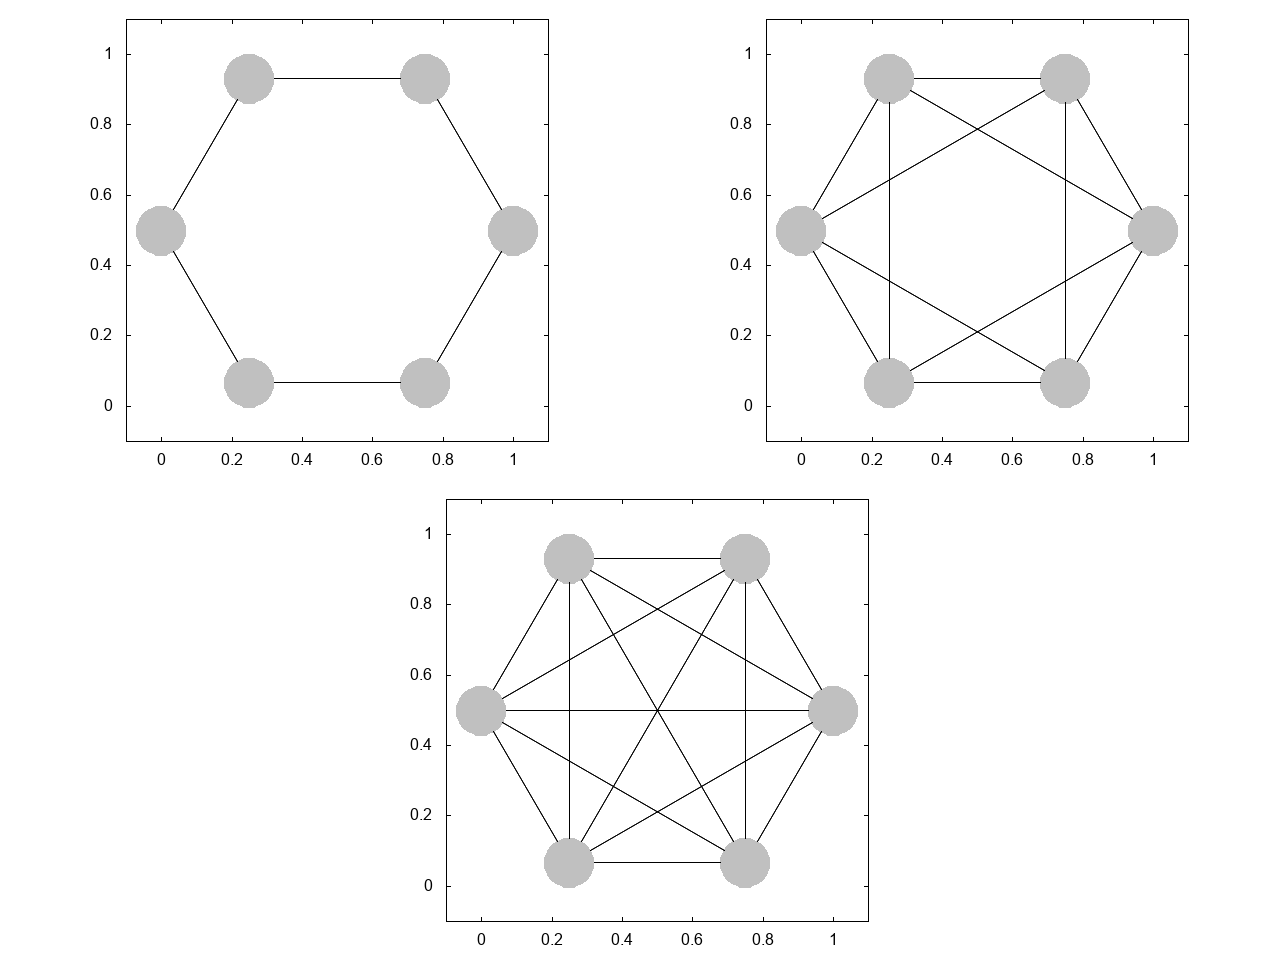
\includegraphics[width=1\textwidth]{grafoEjemplo6}
    \centering
    \caption{En orden izquierda, derecha y abajo, grafos de seis nodos con $k = \{ 1, 2, 3 \}$ y $\{ 6, 12, 15 \}$ aristas.}
    \label{grafoEjemplo6}
  \end{figure}

  

  %\bibliography{biblio}{}
  %\bibliographystyle{plain}

\end{document}
